\section{\huge{Bonusopgaver}}
(til de flittige snapsedrikkere)


\subsection{Opgave 0 skal erstattes}
Udtryk funktionen \texttt{foldl} udelukkende ved hjælp af
\texttt{foldr} og uden eksplicit rekursion.
Husk at \texttt{foldr} og \texttt{foldl} i SML begge har typen
\begin{verbatim}
('a * 'b -> 'b) -> 'b -> 'a list -> 'b
\end{verbatim}


\subsection{Opgave 1 - soerend edit}
Donald skal købe julegaver og betaler 1,- pr. kg. Der er 5 forskellige
pakker: A, B, C, D. Han skal have en af hver, men kan ikke huske hvad de
forskellige gaver vejer. Han kan dog huske hvad nogle kombinationer af gaverne
vejer:

\begin{align*}
2A + 2B + C + 3D &= 54kg \\
4B + C &= 23kg \\
4A + 2C + 5D &= 84kg \\
A + B + 3D &= 30kg \\
\end{align*}

Hvor meget skal Donald betale for én af hver?

% Alle tallene bliver positive, og der er en entydig løsning. Fisse!

%Løs ligningssystemet  $f(\vec{x}) = (8, 7, 32)$, hvor $f : \mathbb{R}^3 → \mathbb{R}^3$ er givet ved
%$$
%f \begin{pmatrix}
%	x_1 \\
%	x_2 \\
%	x_3 \\
%\end{pmatrix} = 
%\begin{pmatrix}
%	4x_2+16x_3 \\
%	x_1-2x_2+7x_3 \\
%	4x_1-6x_2+36x_3 \\
%\end{pmatrix} 
%$$


\subsection{Opgave 2 skal erstattes}
Omskriv tallet 74,7 til dets 32-bit IEEE 754 repræsentation. Blev
der mistet præcision?

\subsection{Opgave 3}
Konstruer en SLR-parsertabel for følgende grammatik:

\[
S \rightarrow \texttt{torben}\ S'\ \texttt{og}\ \texttt{fritz}
\]
\[
S \rightarrow \texttt{torben}\ F\ \texttt{og}\ \texttt{torben}
\]
\[
F \rightarrow S''\ \texttt{fritz}\ S''\ \texttt{fritz}\ S\ |\ \texttt{torben}\ \texttt{, }\ F
\]
\[
S' \rightarrow \epsilon\ |\ \texttt{, }\ S
\]
\[
S'' \rightarrow \texttt{, }\ |\ \texttt{, }\ S\ \texttt{, }
\]
\subsection{Opgave 4}
Som storkunde hos internetudbyderen IP Factory har du har fået tildelt IP-adresseblokken 200.23.18.0/23.
Hvor mange forskellige IP-adresser råder du over? Angiv også den højeste og den laveste IP-adresse i dit råderum.

\subsection{Opgave 5}
Hvilken af nedenstående farver er mest brugervenlig?
\begin{center}
\hspace*{.5cm} 1. engleblå \hspace*{.5cm} 2. koboltblå \hspace*{.5cm} 3. azurblå\hspace*{.5cm}
\end{center}
Skriv derefter en 70-siders rapport hvori du diskuterer designet af et valgfri
it-system som benytter den mest brugervenlige farve.
Referer relevant litteratur hvor du kan finde plads!

\subsection{Opgave 6}
Kig på sætningen:

\begin{center}
\emph{Everybody loves my baby,\\ but my baby loves nobody but me.}
\end{center}

Brug deduktion til at vise, at ovenstående påstand medfører at
\textit{my baby = me}.

\subsection{Opgave 7}
Håndkør følgende Whitespace-program og rapportér dets output:
\begin{verbatim}
   					   
	
     		 		  
	
     	 	 
	
  



\end{verbatim}

\subsection{Opgave 8}
Donald arbejder på et stort universitet hvor folk køber gaver til hinanden.
Det er dog ikke alle der køber gaver til hinanden. Donald har samlet information
om dette og fundet frem til, at der er $N$ personer og $M$ par af personer, der
køber gaver til hinanden. Han ved dog ikke hvem disse $M$ par er.

Donald er interesseret i at finde den mindst mulige størrelse af den største
gruppe af personer der alle køber gaver til hinanden.

Beskriv en algoritme der kan finde størrelsen på denne klike i $O(\lg N)$
tid.

Herunder ses et eksempel med $8$ personer og $10$ gavepar. Den største klike
i eksemplet har størrelse $4$, men det er større end løsningen for $N = 8, M=10$.

% Brug Thurans theorem og binær søgning i n.
% Turans theorem: slå op på wiki.

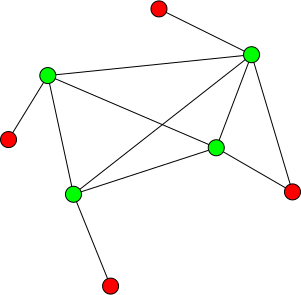
\includegraphics[width=0.7\columnwidth]{turangraph}

\subsection{Opgave 9}
Find det mindste talpar $m,n \in \mathbb{N}$ for hvilket det gælder
$$
m!+1=n^2\quad,\quad m>7\quad,\quad n>7
$$

\textbf{\emph{NB: Der udloddes en flaske snaps til den første som kommer op i baren med en korrekt besvarelse af denne opgave!}}



